\section{Act 1: Designing and analyzing a typical ET experiment in our field }
\subsection{The core four of a 2x2 VWP experiment}
The development of the visual world paradigm (VWP) to study real-time language processing is fundamentally tied to at least two findings: eye-movements have a close relationship with discourse topics \parencite{Cooper} and looks to visual stimuli are sensitive to fine grained phonetic differences over time (e.g., beetle-beaker/ breaker-speaker) \parencite[e.g.][]{Tanenhaus_Spivey-Knowlton_Eberhard_Sedivy_1995,Allopenna_1998}. The now classic VWP design involves a 2x2 design including a target, competitor(s), and distractor(s) with a variety of possible formats from pictures to words. As seen in figure \ref{fig:core_four}, in the VWP a set of images are displayed on a screen time locked to a point in an audio file (e.g., beaker). Both previewing and delayed presentation of images is common. Ultimately, the specific timing used in a study depends on the design  \parencite[see,][, for a review]{Apfelbaum_Klein-Packard_McMurray_2021}{}{}.  The participant then either needs to select the correct answer based on the audio that they perceived or simply listen in look as the sound stimuli plays (e.g., passive listening). VWP experiments vary widely in what linguistic process is being investigated (e.g., referent prediction, sentence processing, word recognition, phonetic cue integration). However, all VWP experiments carefully control three core variables (i.e., time, audio stimuli, and visual stimuli) in order to bring meaning to a fourth core construct: eye-fixations. 

\begin{figure}[ht]
    \centering
    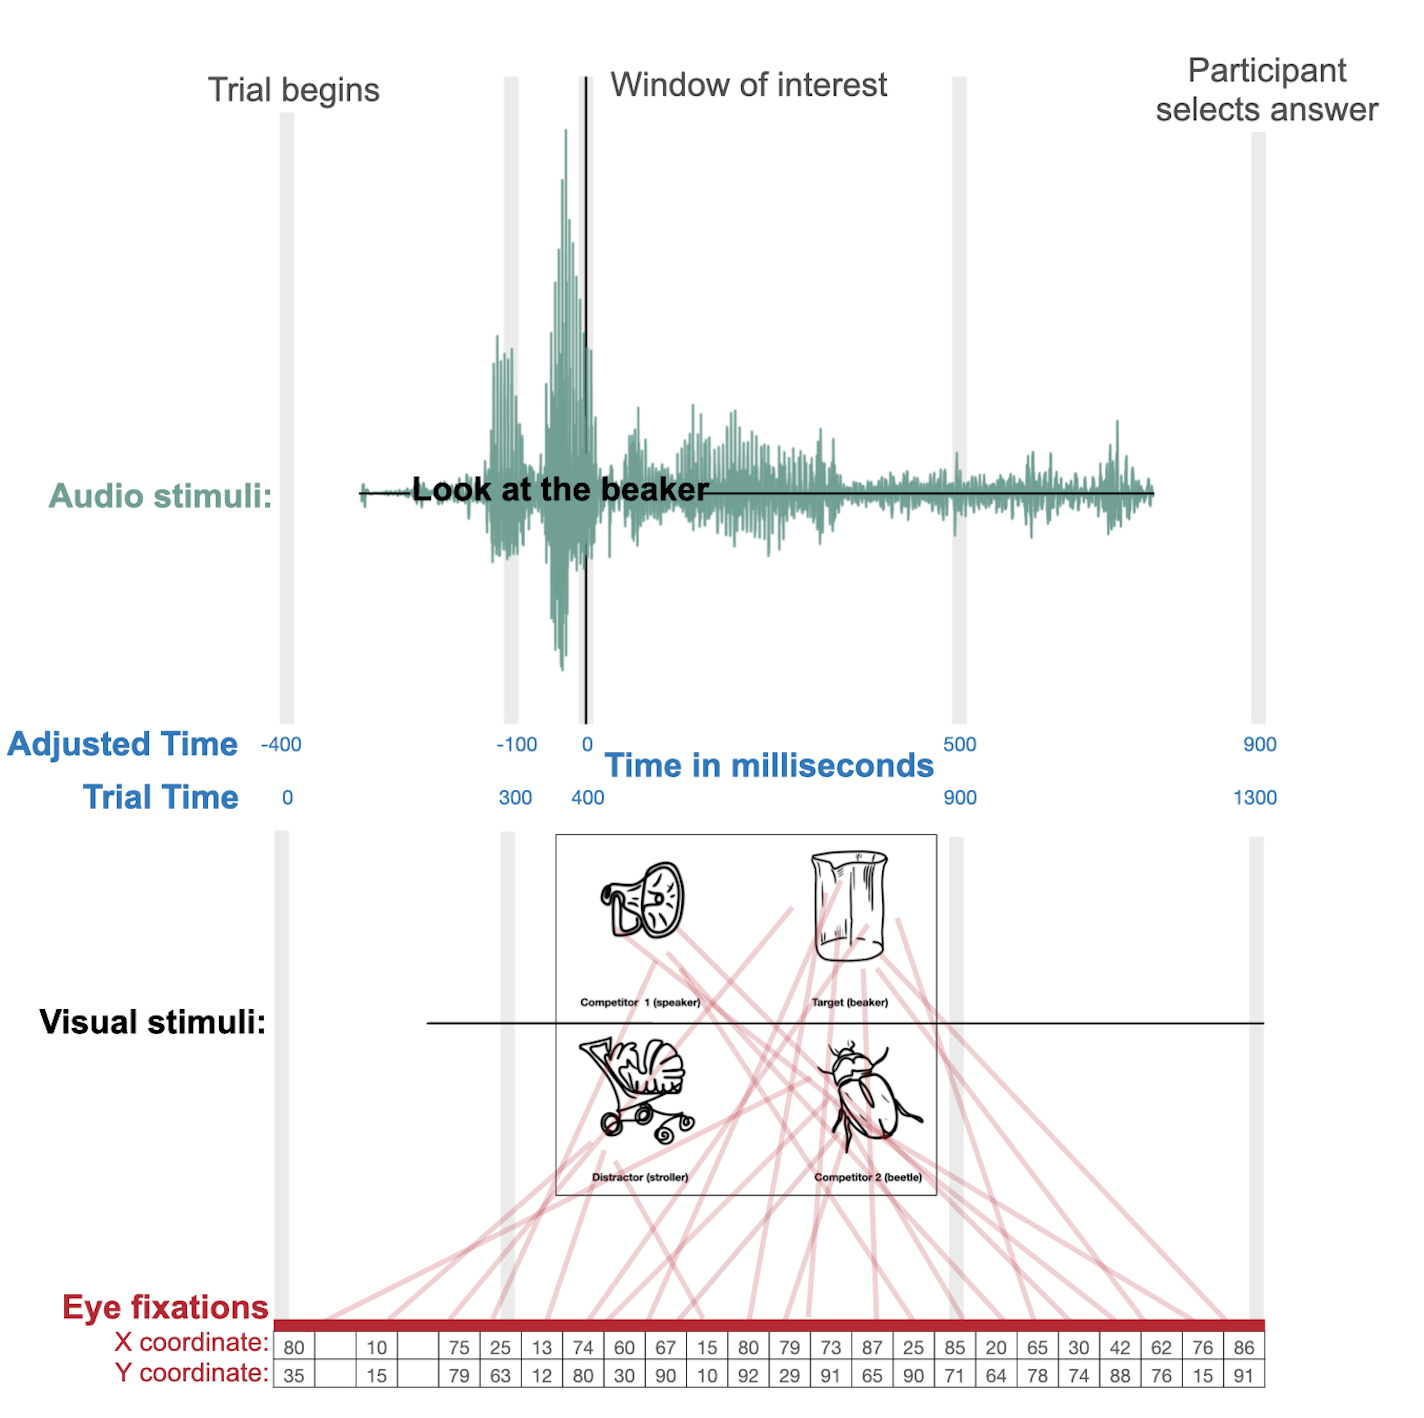
\includegraphics[scale=.6]{figures/core_four}
    \caption{A basic illustration of the core four constructs of the VWP. }
    \label{fig:core_four}
\end{figure}

For the remained of this paper, these "core four" constructs will be used to guide the reader's understanding of how variation in eye-movement behavior can be captured, organized, and analyzed. 

\textbf{Time.} Eye-tracking is especially valuable, in part, because it is an online measure that provides the time-course of processing. Time can be measured from the beginning of the trial to the end of the trial. There are two adjustments, however, that are often made to the time variable. First, it typically takes a listener about 200 ms to plan an eye-movement \parencite[][]{Matin_Shao_Boff_1993}. Eye-movements within the first 200 ms are therefore meaningless and researchers typically account for this 200 ms delay by adjusting the analysis. Second, within each trial there exists a  window of interest, which is only a portion of the full trial time corresponding to post-audio stimui presentation. For example, time in which any carrier phrase is presented is typically ignored and time after the start of the target word is examined. As a result, trial time is often converted to an adjusted time.

\textbf{Audio Stimuli.} are usually grouped into conditions by a separate variable(s) (condition(s)) . Where one variation is expected to illicit one type of behavior and another is expected to illicit a different behavior. The audio segment can be a word, a sentence, or even a non-speech noise. The audio reveals which of the visual stimuli is the correct answer. 

\textbf{Visual Stimuli:} are minimally made up of two types: targets and competitors. In the case of 4 visual stimuli an additional two visual stimuli usually include either a second competitor and a single distractor or two distractors (if a second competitor is not built into the design). Visual stimuli should not be confused with quadrants which are absolute position on the computer screen (e.g., upper right, upper left, bottom left, bottom right). Visual stimuli are always counterbalanced into all possible quadrants so as to reduce the chances of bias in eye-movements. 

\textbf{Eye-Fixations:} are where participants are looking at a particular time. Said another way, eye-fixations are x, y coordinates on the screen that are recorded throughout a trial. The rate of recording is a function of the measurements recorded per second (e.g., measuring 1000 times in one second = 1000Hz) . Eye-fixations get categorized into absolute positions on the screen (quadrants) and then mapped to visual stimuli.

\subsection{Gorilla and data structure}

To run an eye-tracking experiment in Gorilla, a basic forced alternative choice task can serve as the foundation with four visual stimuli as the choices. We must also add a sound stimuli that plays at a specific point in the experiment. Specifically, each trial should start with a fixation cross, afterward provide an initial exposure to visual stimuli for a set period of time (e.g., 200 ms), followed by an audio stimuli playing. The audio stimuli will either provide suggestive hints toward a specific visual stimuli or even explicitly tell the participant which to choose. When building the experiment, it is essential to focus on the timing of the trials, the types of data you want out of the trial, and when the webcam should track eye-fixations. 

The eye-tracker 2 from Gorilla has two explicit modes: calibration and recording. Calibration can be used throughout the experiment or only once at the beginning of the experiment. Additionally, two types of calibration standards can be used, five-point and nine-point, with any level set for calibration fail points or repeat calibrations. Nine-point calibration provides a better standard but takes longer and may fail more often. While not fully necessary because of the manner that webgazer.js functions \parencite[e.g.,][]{ Chen_et_al_2001}, it is highly recommended that the researcher uses calibration throughout the experiment. However, our experiment did not use a calibration requirement and still successfully captured predictive eye-movements \parencite[][]{Prystauka_Altmann_Rothman_2023}. The recording screen is for the experiment trials themselves. The first screen that you want the eye-tracker to start will nearly always be where the visual stimuli begins. Crucially, in the settings, selecting continue tracking on next display and collect detailed eye-tracking data are essential. All screen you wish to record eye-fixations for should also have an eye-tracker module. Basic eye-tracking data and detailed eye-tracking data are different in that basic data does not provide time course data. 

Unlike the eye-link 1000 (used in \parencite{Porretta_et_al_2020}), which measures at 1000 hz, webcams have variable frame rates that depend on the lighting, participant movement, and the participants device, which can range between 20hz and 60hz \parencite{Vos_2017}. Simply put, the raw amount of eye-fixations captured per second is maximally 60, but likely much lower in most cases. Additionally, the environment of the participant also has a strong effect. For example, darker rooms will lead to the camera capturing less eye fixation per second (lower fps). This means that some trials will capture more eye-fixations than other trials. \parencite{} Additionally, the timing of eye-fixations can vary within a trial with non-equal measurements between captured eye fixations. On the aggregate, this mean that the eye-fixations being captured starts to drop throughout the trial. This variability in frame rate can be somewhat attenuated by doing in person eye-tracking with web-gazer but is non-the less somewhat unavoidable \parencite[e.g.,][]{}{}{}. 

Raw data from a VWP experiment downloaded from Gorilla has two basic parts: behavioral data by node and an \textit{uploads} folder (trial by trial specific data for each participant). This format is not limited to eye-tracking data and is true for any experiment that would need additional trial specific data (e.g., voice recordings, mouse-tracking) beyond simple behavioral responses (e.g., reaction time, accuracy). Behavioral data will include all selections and timing of those selections (e.g., reaction time, condition, trial order). However, the additional an uploads folder will contain trial by trial eye-fixation data that is paired with within trial trial-time.  A simplified example of this is shown in figure \ref{fig:data_structure}. The amount of behavioral data sheets has a direct relationship with the number of experimental (and/or questionnaire) nodes in your experiment. While it depends on your design, if counterbalancing audio stimuli by conditions so that participants do not hear the same audio from two speakers, then each of these will also have there own node. That is, if you were to have four counterbalanced stimuli spreadsheets in your experiment design then you will have four raw behavioral data sheets, one from each of these nodes. However, the number of spreadsheets in the upload data folder will depend on how many participants and trials you have. For example, if you have 60 participants who finish 50 trials, you will have a total of 3,000 eye-tracking data sheets (50X60) that reference the behavior trials in your four behavioral data sheets.

\begin{figure}[ht]
    \centering
    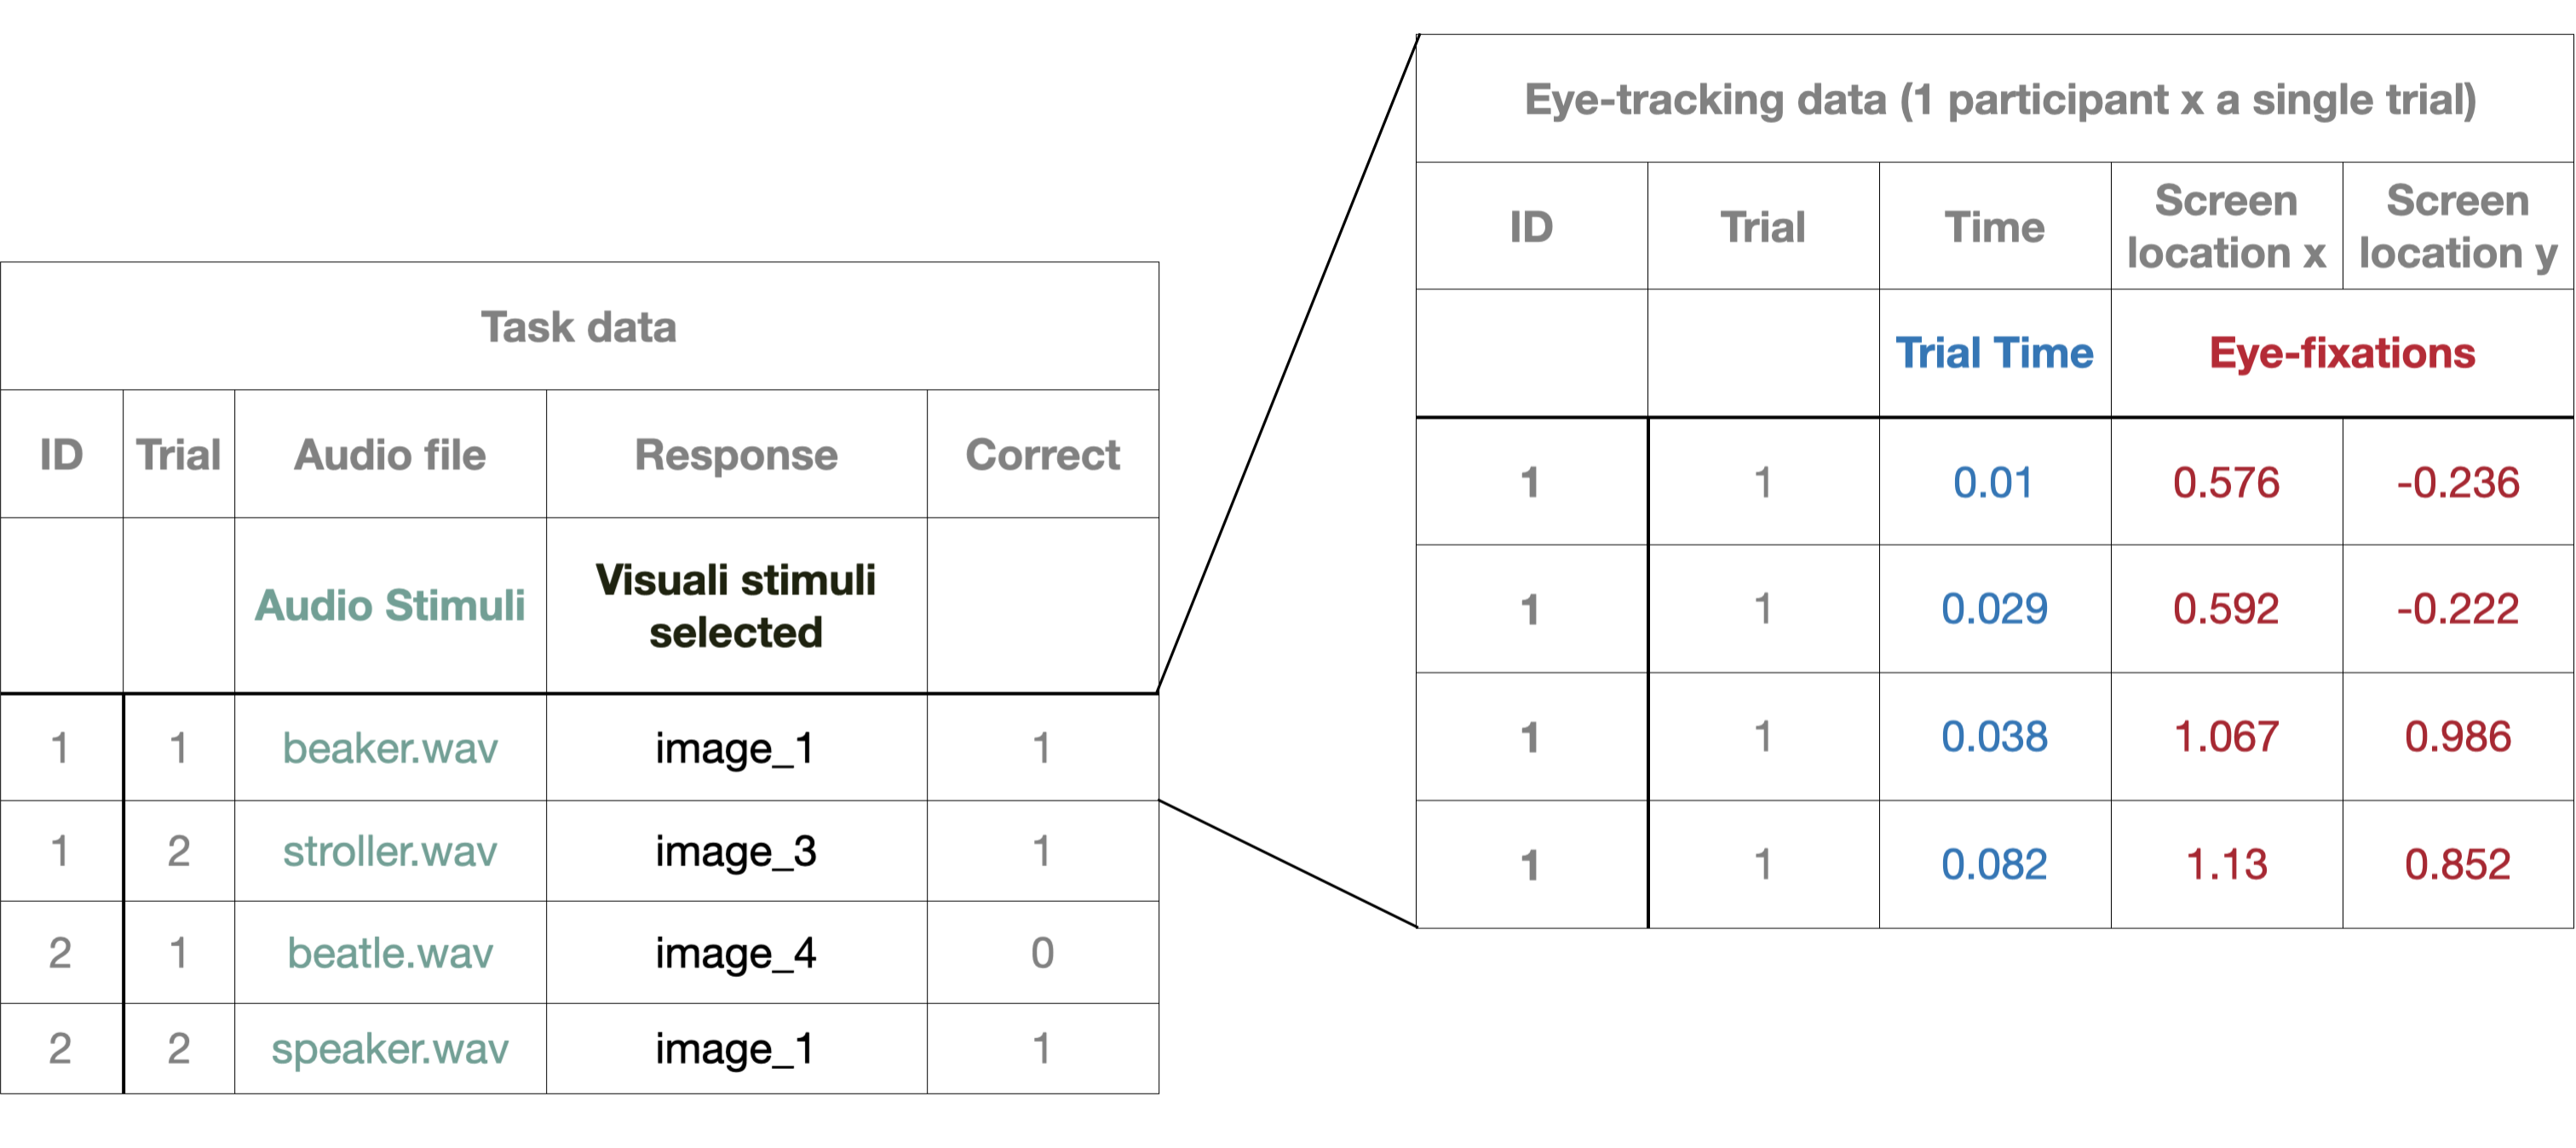
\includegraphics[scale=.2]{figures/data_structure.png}
    \caption{behaviorial data (left) and trial by trial eye-tracking data (right)-\textit{uploads} data. Colors match figure \ref{fig:core_four} layout for ease.}
    \label{fig:data_structure}
\end{figure}

The raw data that Gorilla provides is maximally informative to enable a variety of experiments and analyses to be done. However, this also means that the data is messy. Tidy data is data where each column refers to a single variable (e.g., age) and each row is exactly one observation (e.g., 42). However, what one observation means varies depending on your question. For example, if you are examining questionnaire data, it is likely that each row should have the answer to many questions, where each question is a single column. However, if you are looking at behavioral data then each row show be a different trial for each participant with their response as a single observation. The ways that data can be thought of for tidying will be shown in examples below.





